\classheader{2018-06-20}
\underline{\Large New Question:} Suppose $y'=f(t,y)$, $f$ is \underline{ONLY} a function of y, but $\dfrac{1}{f(y)}$ is hard to integrate. How to study? $\boxed{\frac{1}{f(y)} \dfrac{dy}{dt} = 1}$\\
Here $y'=f(y)$ is called \underline{autonomous} ($t$ is not explicit in equation.)
\begin{example-N}
	\begin{equation*}
		\dot{x} = x^{\frac{2}{3}}, \quad y'=Ky, \quad \dfrac{dz}{dt} = z(1-z)
	\end{equation*}
	Then the solution curve will not depend on the starting time, only on the elapsed time. In the slope field, every vertical slice looks the same.\\
	Every horizontal slice is an isocline: a curve along which the slumps of the solution curves are the same.
	\begin{center}
	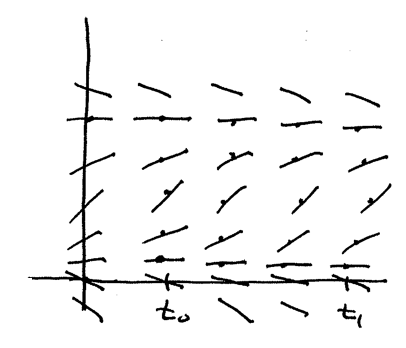
\includegraphics{6-1}\\
		Slopes along every vertical slice look like every other vertical slice. Slopes along every horizontal slice not very.
	\end{center}
\end{example-N}
\begin{enumerate}[label=\protect\circled{\Roman*}]
	\item Existence and uniqueness is determined by continuit of $f$ in $g$ and cont of $\dfrac{df}{dy}$ (not a partial here). 
	\item At any place, $y_0$ where $f(y_0) = 0$, then $y'(t) = 0$ and $y(t) = y_0$ is a \underline{constant solution}. Called an \underline{equilibrium solution}, its graph is horizontal and is an isocline.
		\begin{equation*}
			\dfrac{dz}{dt} = z(1-z). \quad \dfrac{dz}{dt} = 0 \quad \text{ when } z=0,1
		\end{equation*}
		\begin{equation*}
			\text{Hence } z(t) = 0 \text{ is a solution}
		\end{equation*}
		\begin{equation*}
			\text{Hence } z(t) = 1 \text{ is a solution}
		\end{equation*}
		\begin{center}
			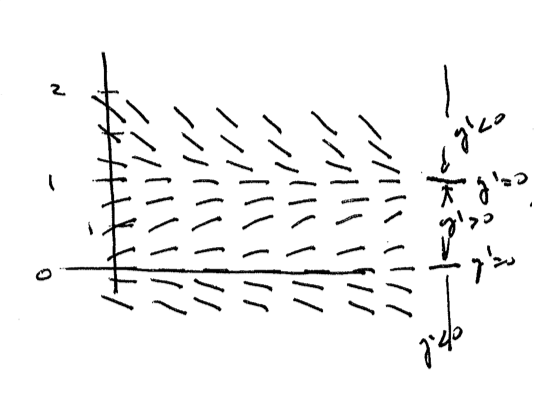
\includegraphics{6-2}
		\end{center}
	\item Outside of the equilibria solutions, of the "sign" of $\dfrac{dz}{dt}$ does not change, hence solutions stock between equilibria will have slopes always negative or always positive.\\
	{\small \textit{\underline{Note:} Without solving, you know pretty much everything. In fact, the slope field is too much information!}}
	\item One vertical slice through the slope field gives you all relevant info. For $z' = f(z) = z(1-z)$
	\begin{center}
	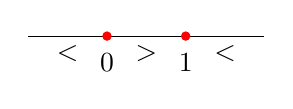
\begin{tikzpicture}
		\draw (-1,0) -- (2,0) ;
		\foreach \i in {0, 1}
			\draw (\i,0.1) circle + (0,-0.2) node[below] {$\i$};
		\foreach \i in {0, 1}
			\fill[red] (\i,0) circle (0.6 mm);
		\foreach \i in {-0.5, 1.5}
			\draw (\i,0.1) circle + (0,-0.1) node[below] {$<$};
		\foreach \i in {0.5}
			\draw (\i,0.1) circle + (0,-0.1) node[below] {$>$};
	\end{tikzpicture}
	\begin{center}
		Sign of $z'$ between equilibria
	\end{center}
	\end{center}
	This is called a \underline{phase line} (think of the y-axis slice in the ty-plane. It is a schematic that gives long term behavior of an autonomous 1st order ODE).
	\begin{example-N}
		Consider $z' = z(1-z), z(0) = \frac{3}{4}$.\\
		Without solving, we know by phase line that $\quad \lim_{t \to \infty } z(t) = 1 $
	\end{example-N}
	In fact, we know the long term behavior of all solutions.
	\begin{equation*}
	\lim_{t \to \infty}z(t) = 
		\begin{cases}
			-\infty & z(0) < 0\\
			0 & z(0) = 0\\
			1 & z(0) > 0
		\end{cases}
	\end{equation*}
	Without a slope field, one can simply graph $f(z)$.\\
	\begin{center}
	 Here on $(-\infty,0), \quad f(z) < 0, \quad z'<0$ for solutions.\\
	 Here on $(0,1), \quad f(z) > 0, \quad z'>0$ for solutions.\\
	   Here on $(1,\infty), \quad f(z) > 0, \quad z'<0$ for solutions.\\	
	\end{center}
	\begin{center}
	\begin{tikzpicture}
		\begin{axis}
		[xmin=-1, xmax=2,
		ymin=-1, ymax=0.6,
		axis lines=center,
		axis on top=true,
		domain=-1:4,
		xlabel={$x$},
    	ylabel={$y$},
    	samples=100]
		\addplot[mark=none, draw=black, thin]{x*(1-x)};
		\node[anchor=south] at (axis cs:0.5,0.3) {$f(z)$};
		\node[anchor=south] at (axis cs:1.5,0.3) {$z(1-z)$};
		\node[anchor=south, color=red] at (axis cs:-0.5,0.05) {$<$};
		\node[anchor=south, color=red] at (axis cs:0.5,0.05) {$>$};
		\node[anchor=south, color=red] at (axis cs:1.5,0.05) {$<$};
		\end{axis}
	\end{tikzpicture} 
	\end{center}
	\item We can use the the seaword derivative test to say more:\\
	$y' = f(y)$ for a solution, then $y'' = f'(y)y'$ helps to determine concavity of infection.\\
\end{enumerate}
\underline{Det:} For $y' = f(y)$, the set $\{y \in \mathbb{R} | f(y) = 0\}$ is the set of critical points for the ODE (equilibrium solutions).\\
Classification of critical points.
\begin{equation*}
	\text{let } y_{\star} \text{ be critical for } y'=f(y) \text{ and call } N_{\varepsilon}(y_{\star}) = \{ y \in \mathbb{R} | |y-y_{\star}| < \varepsilon  \} 
\end{equation*}
\begin{enumerate}[label=\protect\circled{\alph*}]
	\item If $\exists \varepsilon > 0 \text{ where } \forall y \in N_{\varepsilon}(y_{\varepsilon})$ and $\lim_{t \to \infty} y(t) = y_{\star} \Rightarrow y_{\star}$ is asymptotically stable.
	\item If $\exists \varepsilon > 0 \text{ where } \forall y \in N_{\varepsilon}(y_{\varepsilon})$ and $\lim_{t \to -\infty} y(t) = y_{\star} \Rightarrow y_{\star}$ is unstable.
	\item If stable on one side and unstable on other, semi-stable.\\
	\begin{center}
		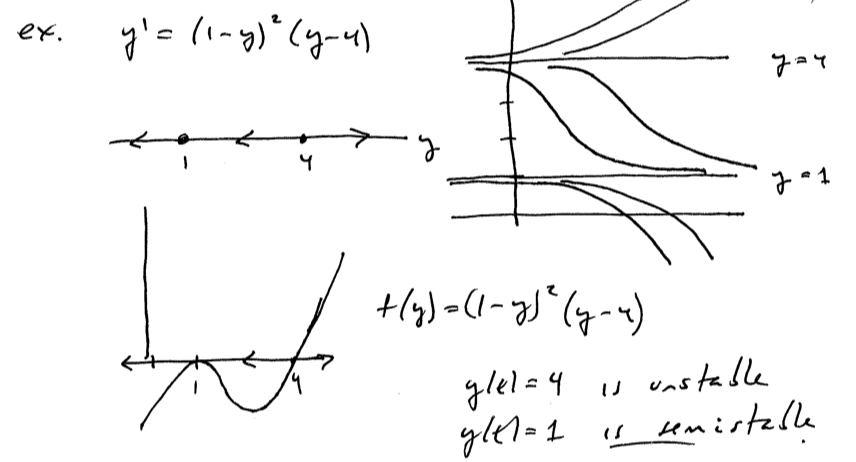
\includegraphics{6-3}		
	\end{center}	
\end{enumerate}